\documentclass{beamer}\usepackage[]{graphicx}\usepackage[]{color}
%% maxwidth is the original width if it is less than linewidth
%% otherwise use linewidth (to make sure the graphics do not exceed the margin)
\makeatletter
\def\maxwidth{ %
  \ifdim\Gin@nat@width>\linewidth
    \linewidth
  \else
    \Gin@nat@width
  \fi
}
\makeatother

\definecolor{fgcolor}{rgb}{0.345, 0.345, 0.345}
\newcommand{\hlnum}[1]{\textcolor[rgb]{0.686,0.059,0.569}{#1}}%
\newcommand{\hlstr}[1]{\textcolor[rgb]{0.192,0.494,0.8}{#1}}%
\newcommand{\hlcom}[1]{\textcolor[rgb]{0.678,0.584,0.686}{\textit{#1}}}%
\newcommand{\hlopt}[1]{\textcolor[rgb]{0,0,0}{#1}}%
\newcommand{\hlstd}[1]{\textcolor[rgb]{0.345,0.345,0.345}{#1}}%
\newcommand{\hlkwa}[1]{\textcolor[rgb]{0.161,0.373,0.58}{\textbf{#1}}}%
\newcommand{\hlkwb}[1]{\textcolor[rgb]{0.69,0.353,0.396}{#1}}%
\newcommand{\hlkwc}[1]{\textcolor[rgb]{0.333,0.667,0.333}{#1}}%
\newcommand{\hlkwd}[1]{\textcolor[rgb]{0.737,0.353,0.396}{\textbf{#1}}}%

\usepackage{framed}
\makeatletter
\newenvironment{kframe}{%
 \def\at@end@of@kframe{}%
 \ifinner\ifhmode%
  \def\at@end@of@kframe{\end{minipage}}%
  \begin{minipage}{\columnwidth}%
 \fi\fi%
 \def\FrameCommand##1{\hskip\@totalleftmargin \hskip-\fboxsep
 \colorbox{shadecolor}{##1}\hskip-\fboxsep
     % There is no \\@totalrightmargin, so:
     \hskip-\linewidth \hskip-\@totalleftmargin \hskip\columnwidth}%
 \MakeFramed {\advance\hsize-\width
   \@totalleftmargin\z@ \linewidth\hsize
   \@setminipage}}%
 {\par\unskip\endMakeFramed%
 \at@end@of@kframe}
\makeatother

\definecolor{shadecolor}{rgb}{.97, .97, .97}
\definecolor{messagecolor}{rgb}{0, 0, 0}
\definecolor{warningcolor}{rgb}{1, 0, 1}
\definecolor{errorcolor}{rgb}{1, 0, 0}
\newenvironment{knitrout}{}{} % an empty environment to be redefined in TeX

\usepackage{alltt}

\makeatletter
\def\maxwidth{ %
  \ifdim\Gin@nat@width>\linewidth
    \linewidth
  \else
    \Gin@nat@width
  \fi
}
\makeatother

\definecolor{shadecolor}{rgb}{.97, .97, .97}
\definecolor{messagecolor}{rgb}{0, 0, 0}
\definecolor{warningcolor}{rgb}{1, 0, 1}
\definecolor{errorcolor}{rgb}{1, 0, 0}

\usepackage{alltt}
\usepackage{natbib}
\usepackage{array}
\usepackage[font=small,skip=5pt]{caption}
\usepackage{graphicx}
\usepackage{amsmath}
\usepackage{dsfont}
\usepackage[]{algorithm2e}
\usepackage{amsthm}
\usepackage{amsfonts}
\usepackage{url}
\usepackage{ulem}
\usepackage{afterpage}
\usepackage{bbm}
\usepackage{tikz}
\usepackage{amssymb}
\usepackage{bm}
\setbeamertemplate{caption}[numbered]

\usetheme{Warsaw}
\defbeamertemplate*{footline}{shadow theme}
{%
  \leavevmode%
  \hbox{\begin{beamercolorbox}[wd=.5\paperwidth,ht=2.5ex,dp=1.125ex,leftskip=.3cm plus1fil,rightskip=.3cm]{author in head/foot}%
    \usebeamerfont{author in head/foot}\insertframenumber\,/\,\inserttotalframenumber\hfill\insertshortauthor
  \end{beamercolorbox}%
  \begin{beamercolorbox}[wd=.5\paperwidth,ht=2.5ex,dp=1.125ex,leftskip=.3cm,rightskip=.3cm plus1fil]{title in head/foot}%
    \usebeamerfont{title in head/foot}\insertshorttitle%
  \end{beamercolorbox}}%
  \vskip0pt%
}

\setbeamertemplate{headline}{%
\leavevmode%
  \hbox{%
    \begin{beamercolorbox}[wd=\paperwidth,ht=2.5ex,dp=1.125ex]{palette quaternary}%
    \insertsectionnavigationhorizontal{\paperwidth}{\hskip0pt plus1filll}{\hskip0pt plus1filll}
    \end{beamercolorbox}%
  }
}

\title[Real-Time Variational Density Forecasts]{Real-Time Variational Density Forecasts}
\author[Nathaniel Tomasetti]{Nathaniel Tomasetti}
\date{ }
\IfFileExists{upquote.sty}{\usepackage{upquote}}{}
\IfFileExists{upquote.sty}{\usepackage{upquote}}{}
\begin{document}


\begin{frame}
\titlepage
\centering
Supervised by Catherine Forbes and Anastasios Panagiotelis
\end{frame}


\begin{frame}
\section{Motivation}
\frametitle{Motivation}
\begin{itemize}
\item There is an increasing demand for forecasts of the entire predictive density of the variable of interest.
\item Many time series of interest can operate on a very short time-frame.
\item We aim to provide density forecasts for these high frequency time-series by updating posterior and predictive density estimates as each data point is observed.
\item The algorithm used should scale to multivariate observations driven by complex models with large datasets.
\end{itemize}
\end{frame}


\begin{frame}
\frametitle{Bayesian Computation Techniques}
A popular technique is to sample the posterior distribution with Markov Chain Monte Carlo (MCMC). MCMC:
\begin{itemize}
\item Converges in distribution to the posterior density with enough iterations.
\item Can be very slow, and is hard to parallelise.
\item Scales badly to large datasets.
\end{itemize}
Interest is developing in Bayesian approximations, such as Variational Bayes (VB). VB:
\begin{itemize}
\item Is typically orders of magnitude faster than MCMC.
\item Scales very well to large datasets with subsampling and parallelisation.
\item Has no theoretical guarantee to converge to the posterior.
\end{itemize}
\end{frame}


\begin{frame}
\section{Markov Chain Monte Carlo}
\frametitle{Markov Chain Monte Carlo}
\begin{itemize}
\item A Gibbs MCMC sampler iteratively samples the full conditional distributions:
\begin{align}
&p(\theta_1 | \theta_2, \dots, \theta_k, y_{1:T}) \nonumber \\
&p(\theta_2 | \theta_1, \theta_3, \dots, \theta_k, y_{1:T}) \nonumber \\
&\vdots \nonumber \\
&p(\theta_k | \theta_1, \dots, \theta_{k-1}, y_{1:T}). \nonumber
\end{align}
\item Requires convergence, which can be extremely slow.
\item A predictive density for the next data point may not be available before it is observed.
\end{itemize}
\end{frame}


\begin{frame}
\frametitle{Deriving Gibbs Full Conditional Distributions}
\begin{itemize}
\item Let $y_t \overset{iid}{\sim} \mathcal{N}(\mu, \sigma^2) \mbox{ for } t = 1, 2, \dots, T$. 
\item Use priors $p(\sigma^2) \sim IG(\mbox{shape} = \alpha, \mbox{scale} = \beta), p(\mu | \sigma) \sim \mathcal{N}(\gamma, \sigma^2/\tau)$.
\item Gibbs MCMC requires the distribution $p(\mu_{(i)} | \sigma^2_{(i)}, y_{1:T})$. 
\item Step One: Write the full log joint distribution,
\end{itemize}
\begin{align}
\log(p(y_{1:T}, \mu, \sigma^2)) &=  -(T/2 + \alpha + 2)\log(\sigma^2) - \frac{\sum_{t}(y_t - \mu)^2}{2\sigma^2} \nonumber \\
&- \frac{\tau(\mu - \gamma)^2}{2\sigma^2} - \frac{\beta}{\sigma^2}  + c. \nonumber 
\end{align}
\end{frame}


\begin{frame}
\frametitle{Deriving Gibbs Full Conditional Distributions}
\begin{itemize}
\item Step Two: Ignore components that do not depend on $\mu$ to form $\log(p(\mu | \sigma^2, y_{1:T}))$,
\begin{equation}
\log(p(\mu | y_{1:T}, \sigma^2)) =  - \frac{\sum_{t}(y_t - \mu)^2}{2\sigma^2} - \frac{\tau(\mu - \gamma)^2}{2\sigma^2} + c. \nonumber
\end{equation}
\item Step Three: Condition on the previous draw of $\sigma^2$ to form $\log(p(\mu_{(i)} | \sigma^2_{(i)}, y_{1:T}))$,
\begin{equation}
\log(p(\mu_{(i)} | \sigma^2_{(i)}, y_{1:T})) = - \frac{\sum_{t}(y_t - \mu_{(i)})^2}{2\sigma_{(i)}^2} - \frac{\tau(\mu_{(i)} - \gamma)^2}{2\sigma_{(i)}^2}  + c. \nonumber
\end{equation}
\item Step Four: Manipulate equation until a distribution kernel is recognised. If unrecognised, add a Metropolis-Hastings step.\
\item Step Five: Repeat for $p(\sigma^2_{(i)} | \mu_{(i-1)}, y_{1:T}).$
\end{itemize}
\end{frame}


\begin{frame}
\section{Variational Bayes}
\frametitle{Variational Bayes}
\begin{itemize}
\item Key Idea: Replace the intractable $p(\boldsymbol{\theta} | y_{1:T})$ with a tractable approximation $q(\boldsymbol{\theta} | \boldsymbol{\lambda})$.
\item How: Choose the $q(\boldsymbol{\theta} | \boldsymbol{\lambda})$ from a restricted class of distributions that minimises a well defined divergence between $q(\boldsymbol{\theta} | \boldsymbol{\lambda})$ and $p(\boldsymbol{\theta} | y_{1:T})$. 
\item The classic choice is the Kullback-Leibler divergence from $q$ to $p$,
\begin{equation}
\label{KL-def}
KL[q(\boldsymbol{\theta} | \boldsymbol{\lambda})\hspace{.1cm}||\hspace{.1cm}p(\boldsymbol{\theta} | y_{1:T})] = \int q(\boldsymbol{\theta} | \boldsymbol{\lambda}) \ln \left( \frac{q(\boldsymbol{\theta} | \boldsymbol{\lambda})}{p(\boldsymbol{\theta} |y_{1:T})}\right) d\boldsymbol{\theta}.
\end{equation}
\item (\ref{KL-def}) is non-negative and equals zero if and only if $p(\boldsymbol{\theta} | y_{1:T}) = q(\boldsymbol{\theta} | \boldsymbol{\lambda})$ almost everywhere.
\end{itemize}
\end{frame}


\begin{frame}
\frametitle{The Evidence Lower Bound}
\begin{itemize}
\item Rewrite (\ref{KL-def}) as
\begin{equation}
\label{KL-ELBO}
KL[q(\boldsymbol{\theta} | \boldsymbol{\lambda})\hspace{.1cm}||\hspace{.1cm}p(\boldsymbol{\theta} |y_{1:T})] = \ln(p(y_{1:T})) - \mathcal{L}(q(\boldsymbol{\theta} | \boldsymbol{\lambda}), y_{1:T}),
\end{equation}
where
\begin{equation}
\label{ELBO}
\mathcal{L}(q(\boldsymbol{\theta} | \boldsymbol{\lambda}), y_{1:T}) = \mathbb{E}_{q} \left( \ln (p(y_{1:T},\boldsymbol{\theta})) - \ln (q(\boldsymbol{\theta} | \boldsymbol{\lambda})) \right).
\end{equation}
\item $\mathcal{L}(q(\boldsymbol{\theta} | \boldsymbol{\lambda}), y_{1:T})$ is refered to as the Evidence Lower Bound (ELBO).
\item Maximising the ELBO with respect to $q \iff$ Minimising the KL Divergence with respect to $q$.
\item There are two tasks: 
  \begin{enumerate}
  \item Choose a functional form for $q$. 
  \item Optimise auxillary parameter vector $\boldsymbol{\lambda}$. 
  \end{enumerate}
\end{itemize}
\end{frame}


\begin{frame}
\frametitle{Mean Field Variational Bayes}
\begin{itemize}
\item Early Variational Bayes implementation pioneered by \citet{Jordan1999} and \citet{Ghahramani2000}.
\item Restricts $q(\boldsymbol{\theta} | \boldsymbol{\lambda})$ to the factorisable family,
\begin{equation}
\label{mf1}
q(\boldsymbol{\theta} | \boldsymbol{\lambda}) = \prod_{i=1}^k q_i(\theta_i | \boldsymbol{\lambda_i}).
\end{equation}
\item Restricts the model to the exponential family with conjugate priors.
\item Provides the optimal distribution for each $q_i(\theta_i | \boldsymbol{\lambda_i})$.
\item Maximise the ELBO by setting each factor to
\begin{equation}
\label{mf2}
q_i(\theta_i |\boldsymbol{\lambda_i}) \propto\exp( \mathbb{E}_{\prod_{j \neq i} q_i(\theta_i | \boldsymbol{\lambda_i})} [\ln(p(y_{1:T},\boldsymbol{\theta}))]).
\end{equation}
\end{itemize}
\end{frame}


\begin{frame}
\frametitle{Deriving $q$ distributions}
\begin{itemize}
\item (\ref{mf2}) is applied to the Normal-Inverse Gamma model to find $q(\mu | \boldsymbol{\lambda}_1)$.
\item Step One: Write the full log joint distribution,
\begin{align}
\log(p(y_{1:T}, \mu, \sigma^2)) &= -(T/2 + \alpha + 2)\log(\sigma^2) - \frac{\sum_{t}(y_t - \mu)^2}{2\sigma^2} \nonumber \\
&- \frac{\tau(\mu - \gamma)^2}{2\sigma^2} - \frac{\beta}{\sigma^2} + c. \nonumber 
\end{align}
\item Step Two: Ignore components that do not depend on $\mu$ to form $\log(p(\mu | \sigma^2, y_{1:T})),$
\begin{equation}
\log(p(\mu | y_{1:T}, \sigma^2)) = - \frac{\sum_{t}(y_t - \mu)^2}{2\sigma^2} - \frac{\tau(\mu - \gamma)^2}{2\sigma^2} + c. \nonumber
\end{equation}
\end{itemize}
\end{frame}


\begin{frame}
\frametitle{Deriving $q$ distributions}
\begin{itemize}
\item Step Three: Take the expectation with respect to $q(\sigma^2 | \boldsymbol{\lambda}_2)$ to form $\log(q(\mu | \boldsymbol{\lambda}_1)),$
\begin{equation}
\log(q(\mu | \boldsymbol{\lambda}_1)) = - 1/2 \mathbb{E}_{q(\sigma^2)} [\sigma^{-2}] \left( \sum_{t}(y_t - \mu)^2 + \tau(\mu - \gamma)^2 \right)  + c. \nonumber
\end{equation}
\item Step Four: Manipulate equation until a distribution kernel is recognised. If unrecognised, add a secondary approximation.
\item Step Five: Repeat for $q(\sigma^2 | \boldsymbol{\lambda}_2)$.
\item In this case $q(\mu | \boldsymbol{\lambda}_1) \sim \mathcal{N}(\tilde{\gamma}, \tilde{\tau})$ and $q(\sigma^2 | \boldsymbol{\lambda}_2) \sim IG(\tilde{\alpha}, \tilde{\beta})$.
\end{itemize}
\end{frame}


\begin{frame}
\frametitle{Deriving $q$ distributions}
\begin{itemize}
\item The auxillary parameter vector is $\boldsymbol{\lambda} = (\tilde{\gamma}, \tilde{\tau}, \tilde{\alpha}, \tilde{\beta})$, which maximises the ELBO when
\begin{align}
\tilde{\gamma} &= \frac{\tau \gamma + \sum_{t=1}^{T} y_t}{T + \tau}  \label{mf5} \\ 
\tilde{\tau} &= \left((T + \tau)\mathbb{E}_{q(\sigma^2)}[\sigma^{-2}]\right )^{-1} \label{mf6} \\
\tilde{\alpha} &= (T+1)/2 + \alpha  \label{mf7} \\
\tilde{\beta} &= \beta + 1/2\bigg((\tau + T)\mathbb{E}_{q(\mu)}[\mu^2 ]  \nonumber \\ 
&- 2 \mathbb{E}_{q(\mu)}[\mu ]\left(\sum_{t=1}^{T}y_t + \tau\right) + \sum_{t=1}^{T} y_t^2 + \tau \gamma^2 \bigg). \label{mf8}
\end{align}
\end{itemize}
\end{frame}


\begin{frame}
\frametitle{Deriving $q$ distributions}
\begin{itemize}
\item Substitute in expectations to (\ref{mf6}) and (\ref{mf8}):
\begin{align}
\tilde{\tau} &= \frac{\tilde{\beta}}{\tilde{\alpha}(T + \tau)} \label{mf9} \\
\tilde{\beta} &= \beta + 1/2\left((\tau + T)(\tilde{\gamma}^2 + \tilde{\tau}) - 2 \tilde{\gamma}(\sum_{t=1}^{T}y_t + \tau) + \sum_{t=1}^{T} y_t^2 + \tau \gamma^2 \right)\label{mf10}
\end{align}
\item The circular dependence in (\ref{mf9}) and (\ref{mf10}) and can be resolved with a coordinate ascent algorithm.
\end{itemize}
\end{frame}


\begin{frame}
\frametitle{Fit to simulated data}
\begin{itemize}
\item Marginal posterior densities for the Normal Inverse Gamma model with $N = 100, \mu = 2$ and $\sigma^2 = 1$; hyperparameters are $\gamma = 0, \tau = 1, \alpha = 1$ and $\beta = 1$. 
\end{itemize}
\begin{figure}[h]
\centering
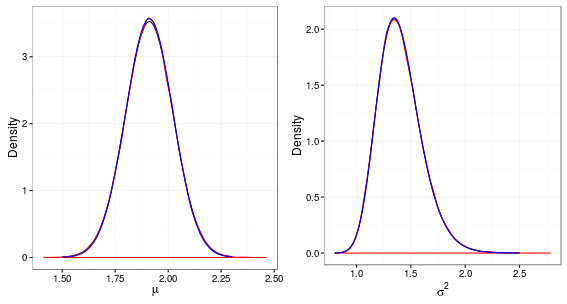
\includegraphics[width=0.7\linewidth,height=\textheight,keepaspectratio]{norminvg}
\caption{The analytical true density (black), the Monte Carlo (red) and the MFVB approximation (blue). MFVB converged in same time as required to take three MCMC samples of each parameter.}
\label{fig:norminvg}
\end{figure}
\end{frame}


\begin{frame}
\frametitle{Stochastic Variational Bayes}
\begin{itemize}
\item \citet{Paisley2012} and \citet{Ranganath2014} adapted a gradient ascent algorithm to maximise the ELBO.
\item Gradient ascent returns the optimal $\boldsymbol{\lambda}$ for a specified functional form $q$.
\item Only requires Monte-Carlo estimates of $\nabla_{\boldsymbol{\lambda}}\mathcal{L}(q(\boldsymbol{\theta} | \boldsymbol{\lambda}), y_{1:T})$,
\begin{align}
\label{SVB}
\nabla_{\boldsymbol{\lambda}}\mathcal{L}(q(\boldsymbol{\theta} | \boldsymbol{\lambda}), y_{1:T}) &\approx \frac{1}{S}\sum_{s=1}^{S} \nabla_{\boldsymbol{\lambda}} [\ln(q(\boldsymbol{\theta}_s | \boldsymbol{\lambda})] \nonumber \\
&\times \big(\ln (p(y_{1:T}, \boldsymbol{\theta}_s)) - \ln(q(\boldsymbol{\theta}_s | \boldsymbol{\lambda}))\big) 
\end{align}
where $\boldsymbol{\theta}_s$ is simulated from $q(\boldsymbol{\theta} | \boldsymbol{\lambda})$ for $s = 1, 2, \dots, S$. 
\end{itemize}
\end{frame}


\begin{frame}
\frametitle{Gradient Ascent}
\begin{itemize}
\item Make steps of the form
\begin{equation}
\lambda^{(m+1)} = \lambda^{(m)} + \rho^{(m)} \nabla_{\lambda} f(\lambda^{(m)})
\end{equation}
until $| f(\lambda^{(m+1)}) - f(\lambda^{(m)}) | < \epsilon$, with $\rho^{(m)}, m = 1, 2, \dots$ that satisfies the \citet{Robbins1951} conditions.
\end{itemize}
\begin{figure}[h]
\centering
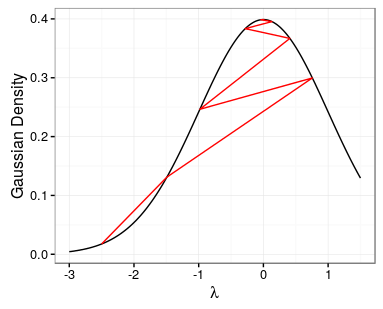
\includegraphics[scale = 0.4]{gradientascent}
\caption{Red steps show the path a variable $\lambda^{(m)}$ took while finding the maximum of a standard normal distribution.}
\label{fig:GradAscent}
\end{figure}
\end{frame}


\begin{frame}
\section{Copulas}
\frametitle{Vine Copulas}
\begin{itemize}
\item Vine copulas allow distributions to be constructed where a flexible dependence structure is fit independently to the margins.
\vspace{3mm}
\item Problem: There are $O(k!)$ ways to construct a vine copula for a $k-$dimensional parameter vector $\boldsymbol{\theta}$.
\item Solution: Di{\ss}mann's algorithm generates a vine copula that fits a sample of data reasonably well.
\item Implementation: Run MCMC and use Di{\ss}mann's algorithm to find a good vine copula to use as $q(\boldsymbol{\theta} | \boldsymbol{\lambda})$. Run SVB to update this approximation as more data comes in.
\end{itemize}
\end{frame}


\begin{frame}
\frametitle{AR2 Model Fit}
\begin{itemize}
\item Simulate an AR(2) with: $T = 150, \phi_1 = 0.7, \phi_2 = 0.2$, and $\sigma^2 = 1$.
\item Run Metropolis-Hastings-within-Gibbs MCMC, select $q$ marginals by BIC from draws, apply Di{\ss}mann's algorithm.
\item Result: $q(\phi_1, \phi_2) = \mbox{BVN}(\boldsymbol{\mu}, \Sigma)$ and $q(\sigma^2) = IG(\alpha, \beta)$. 
\end{itemize}
\begin{figure}[h]
\centering
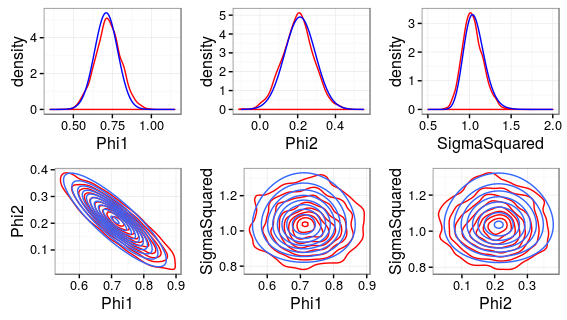
\includegraphics[scale = 0.4]{VBfit.png}
\caption{The fit of an SVB algorithm (blue) compared to MCMC (red) for the AR(2) model. SVB converged in same time as required to take 3000 MCMC samples of each parameter.}
\label{fig:VBfit}
\end{figure}
\end{frame}


\begin{frame}
\section{Empirical Application}
\frametitle{Electricity Load Forecasting}
\begin{itemize}
\item Victorian electricity prices are extremely volatile, and are updated every five minutes.
\item Prices spike electricity load crosses a particular threshold.
\item If we can provide density forecasts for load, we can predict how likely it is for prices to spike in the next period.
\begin{figure}[h]
\centering
\includegraphics[scale = 0.3]{RRP_timeseries.png}
\caption{Half hourly price data for Victoria from January 1 2011 to December 31 2015.}
\label{fig:rrpplot}
\end{figure}
\end{itemize}
\end{frame}



\begin{frame}
\frametitle{Exponential Smoothing}
\begin{itemize}
\item \citet{Taylor2008} provides evidence that a double-seasonal Holt-Winters exponential smoothing model performs better than common alternatives for very short term electricity load forecasting.
\item \citet{Forbes2000} provides a Bayesian approach to estimating exponential smoothing models by Monte Carlo simulation.
\item We slightly modify the Holt-Winters model to work within the Bayesian approach.
\item Applying SVB will allow electricity load density forecasts to be made at a very short time-frame.
\end{itemize}
\end{frame}


\begin{frame}
\frametitle{Double Seasonal Holt-Winters Exponential Smoothing}
\begin{itemize}
\item We use the modified double seasonal Holt-Winters exponential smoothing model
\begin{align}
y_t &= l_{t-1} - \sum_{i = 1}^{m_1 - 1}d_{t-i} - \sum_{i = 1}^{m_2 - 1}w_{t-i} + e_t \label{ds-hw-rp1} \\
l_t &= l_{t-1} + \alpha e_t \label{ds-hw-rp2} \\
d_t &= - \sum_{i = 1}^{m_1 - 1}d_{t-i} + \delta e_t \label{ds-hw-rp3} \\
w_t &= - \sum_{i = 1}^{m_2 - 1}w_{t-i} + \omega e_t \label{ds-hw-rp4}.
\end{align}
where $m_1$ is the length of the daily cycle, and $m_2$ is the length of the weekly cycle.
\item (\ref{ds-hw-rp3}) and (\ref{ds-hw-rp4}) restrict the seasonality but allow us to avoid inverting a singular matrix in the Bayesian approach.
\end{itemize}
\end{frame}


\begin{frame}
\section{Discussion}
\frametitle{Discussion}
\begin{itemize}
\item Updating is worthwhile if the new data brings significant information on the parameters. State-space models are of interest as observation specific latent variables are more influenced by new data than global parameters.
\item Existing online updating algorithms assume data is $iid$. We aim to develop an updating algorithm for dependent data.
\item Our time-series context allows MCMC draws to guide the construction of $q$. We have no information on latent variables associated with new data and we must devise a way to include these in $q$.
\item Statistical properties of the approximation are unknown and depend on the divergence measure used.
\item The accuracy/computation time trade-off between MCMC and VB has not been thoroughly investigated.
\end{itemize}
\end{frame}


\begin{frame}
\frametitle{Timeline}
\begin{itemize}
\item Mid 2017: Complete electricity load forecasting application.
\item End of 2017: Develop dependent online updating, apply to Stochastic Volatiltiy model with dependent latent variables.
\item Compare approximations to the exact posterior to understand the efficiency trade-off.
\item Mid 2018: Investigate statistical properties of other divergence measures such as Stein's discrepancy.
\item End of 2018: Allow extra time as the literature is evolving rapidly and new research opportunities constantly appear.
\item Mid 2019: Finalise thesis for submission.
\end{itemize}
\end{frame}


\begin{frame}
\bibliographystyle{asa}
\bibliography{references}
\end{frame}




\end{document}
